\chapter{Opis rada sistema}\label{sistem}
U ovom poglavlju se detaljno izlaže opis rada sistema iz dve perspektive: perspektive studenta - korisnika sistema, i perspektive profesora - administratora sistema.

\section{Opis rada sistema iz perspektive studenta}
\subsection{Logovanje na sistem i registracija}
Prva stranica koja se prikazuje kada korisnik uputi pretraživač na adresu servisa jeste login stranica (URI: \texttt{/login}), prikazana na slici \ref{fig:login}. Na ovoj stranici korisnik unosi svoju email adresu i lozinku i nakon toga se loguje na sistem pritiskom na dugme \textbf{Prijava}. Prihvataju se samo email adrese koje se završavaju sa \texttt{@etf.rs}. Email adresa se dinamički proverava dok je korisnik unosi, i to tako da je dugme za prijavu onemogućeno dok se ne unese korektna adresa. Pokušaj prijave korisnika koji nije registrovan, ili koji se ulogovao sa pogrešnom lozinkom se prikazuju kao greška (slika \ref{fig:login-error}).

Novi korisnici mogu da se registruju pritiskom na dugme \textbf{Registracija}. Ta akcija ih vodi na stranicu za registrovanje novih korisnika (URI: \texttt{/register}, slika \ref{fig:register}), koja od korisnika traži da unese email adresu. Ista ograničenja vezana za email adresu se primenjuju i ovde. Pokušaj postojećeg korisnika da se ponovo registruje rezultuje greškom. Nakon što unese email, pritiskom na dugme \textbf{Izvrši} se korisnik registruje na sistem. Nakon uspešne registracije korisniku se prikazuje stranica sa slike \ref{fig:register-success}. Tom prilikom se na unetu email adresu automatski šalje email sa nasumično generisanom lozinkom za tog korisnika. Sa ovom lozinkom korisnik sada može da se uloguje na sistem preko stranice za logovanje.
\begin{figure}[p]
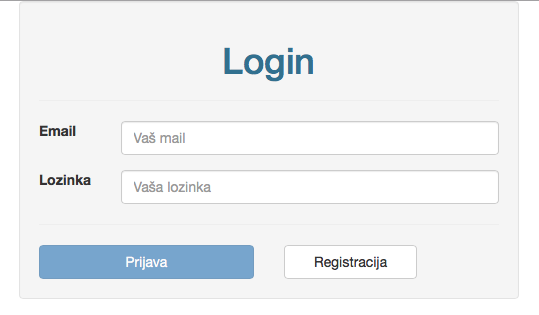
\includegraphics[width=0.5\textwidth]{login}
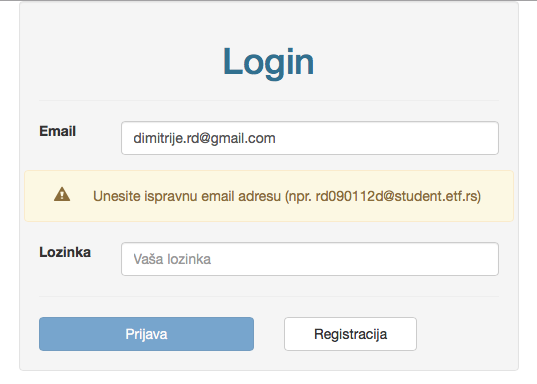
\includegraphics[width=0.5\textwidth]{login-wrongemail}
\caption{Levo: inicijalni izgled login stranice, desno: login stranica tokom unosa email adrese}
\label{fig:login}
\end{figure}
\begin{figure}[p]
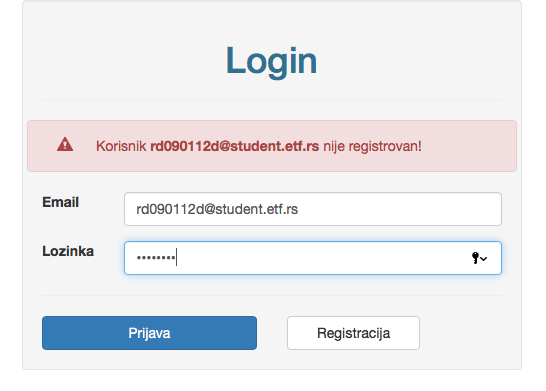
\includegraphics[width=0.5\textwidth]{login-error-unknown}
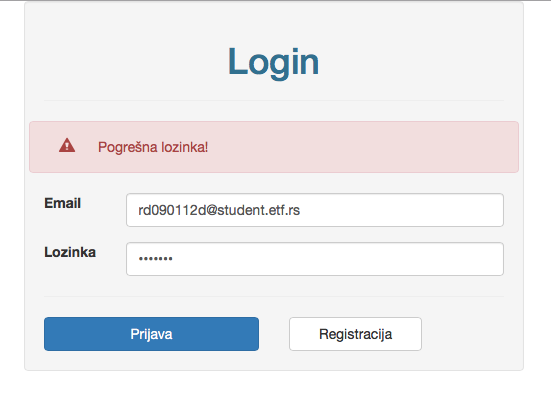
\includegraphics[width=0.5\textwidth]{login-error-password}
\caption{Login stranica nakon što neregistrovani korisnik pokuša da se uloguje (levo), ili ukoliko korisnik unese pogrešnu lozinku (desno)}
\label{fig:login-error}
\end{figure}
\begin{figure}[p]

\includegraphics[width=0.5\textwidth]{register}
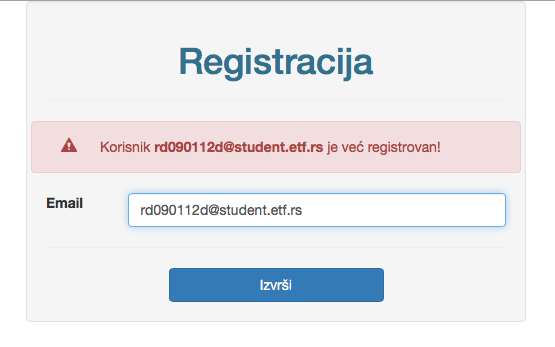
\includegraphics[width=0.5\textwidth]{register-error}
\caption{\textit{Levo}: inicijalni izgled stranice za registrovanje, \textit{desno}: stranica za registracije nakon što već registrovani korisnik pokuša da se registruje}
\label{fig:register}
\end{figure}
\begin{figure}[h]

\includegraphics[width=\textwidth]{register-success}
\caption{Izgled stranice za registraciju nakon uspešne registracije}
\label{fig:register-success}
\end{figure}

\subsection{Stranica sa pregledom testova}
Nakon uspešne prijave na sistem, korisniku se prikazuje stranica sa pregledom svih testova trenutno u sistemu (URI: \texttt{/user}, slike \ref{fig:assignments} i \ref{fig:assignments-collapsed}). Ova stranica se prikazuje i kao početna stranica ukoliko je korisnik već ulogovan na sistem, a pregledač usmeri na \textit{root} URL servisa. Testovi su grupisani po kategorijama, i prikazani unutar tabele u svakoj kategoriji. Zaglavlja tabel sadrže imena kategorija i predstavljaju interaktivne linkove, koji na klik proširuju svoj sadržaj, tj. telo tabele sa testovima.

Za svaki test se prikazuje ime testa, broj stranica sa pitanjima, i ukupan broj pitanja. Testovi koji se prikazuju na ovoj stranici se dele na:
\begin{itemize}
\renewcommand\labelitemi{--}
\item \textbf{Završene testove}, tj. testove koje je korisnik predao. Za ove testove se dodatno prikazuju datum i vreme kada je test započet, datum i vreme kada je test završen, i ocena, u vidu procenta tačnih odgovora u odnosu na ukupan broj pitanja. Boja pozadine ovih unosa je zelena.
\item \textbf{Testove u toku}, tj. testove koje je korisnik započeo, ali nije završio. Za ove testove se dodatno prikazuju datum i vreme kada je test započet, procenat od ukupnog broja pitanja na koja je student dao odgovor, tj. progres, i link ka stranici sa testom. Boja pozadine ovih unosa je žuta.
\item \textbf{Nezapočete testove}, tj. testove koje korisnik nikada nije polagao. Za ove testove se dodatno prikazuje link ka stranici sa testom i prazan progres. Boja pozadine ovih unosa je bela.
\end{itemize}
\begin{figure}[p]
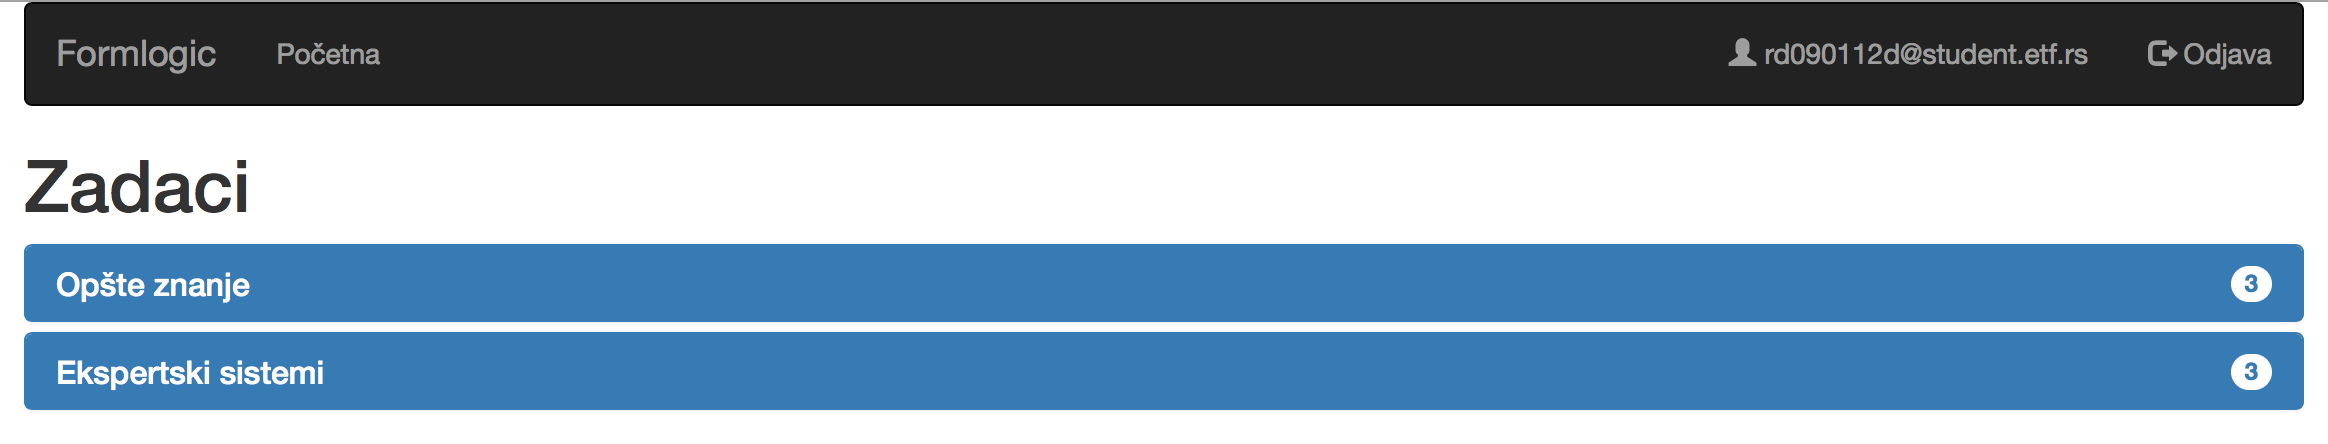
\includegraphics[width=\textwidth]{assignments}
\caption{Inicijalni izgled stranice sa zadacima, sa izlistanim kategorijama (broj testova unutar kategorije je naznačen sa desne strane interaktivnog linka)}
\label{fig:assignments}
\end{figure}
\begin{figure}[p]
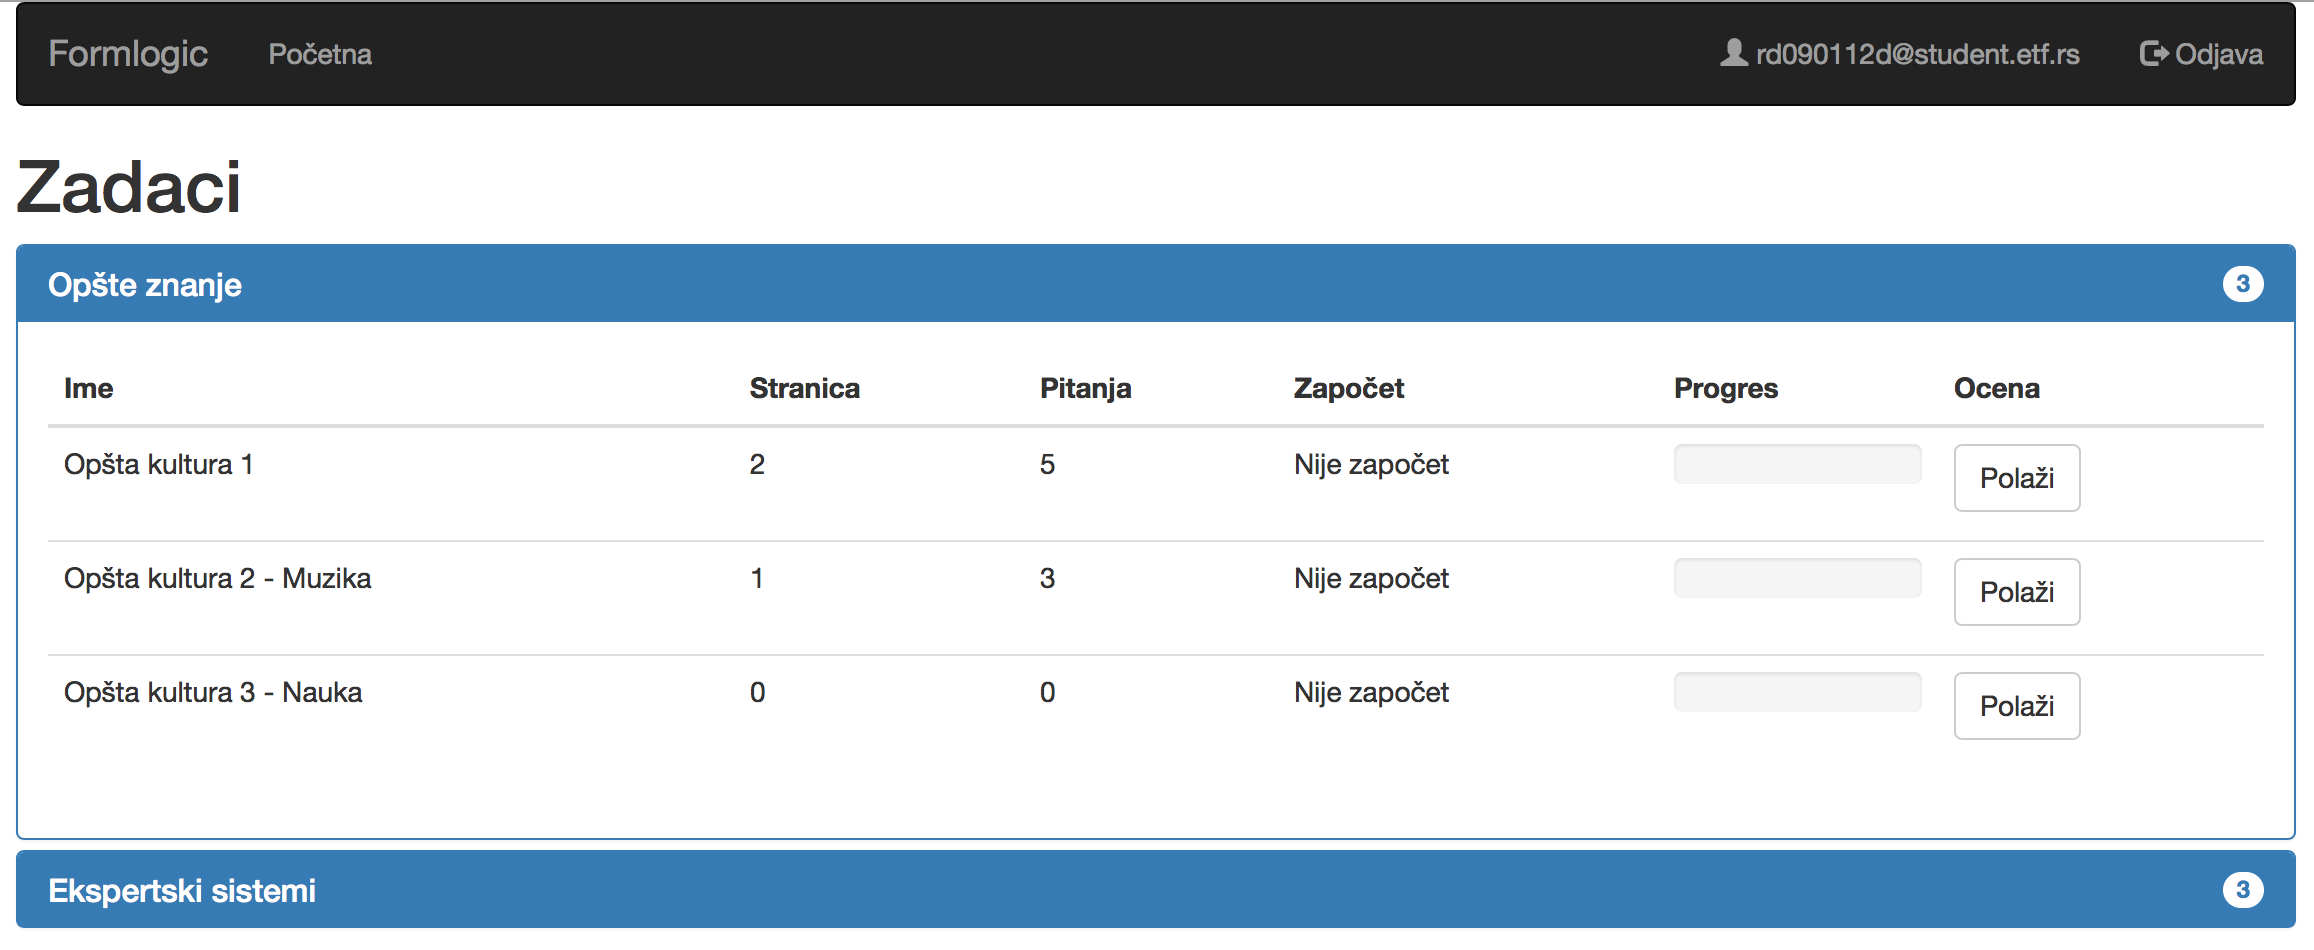
\includegraphics[width=\textwidth]{assignments-collapsed}
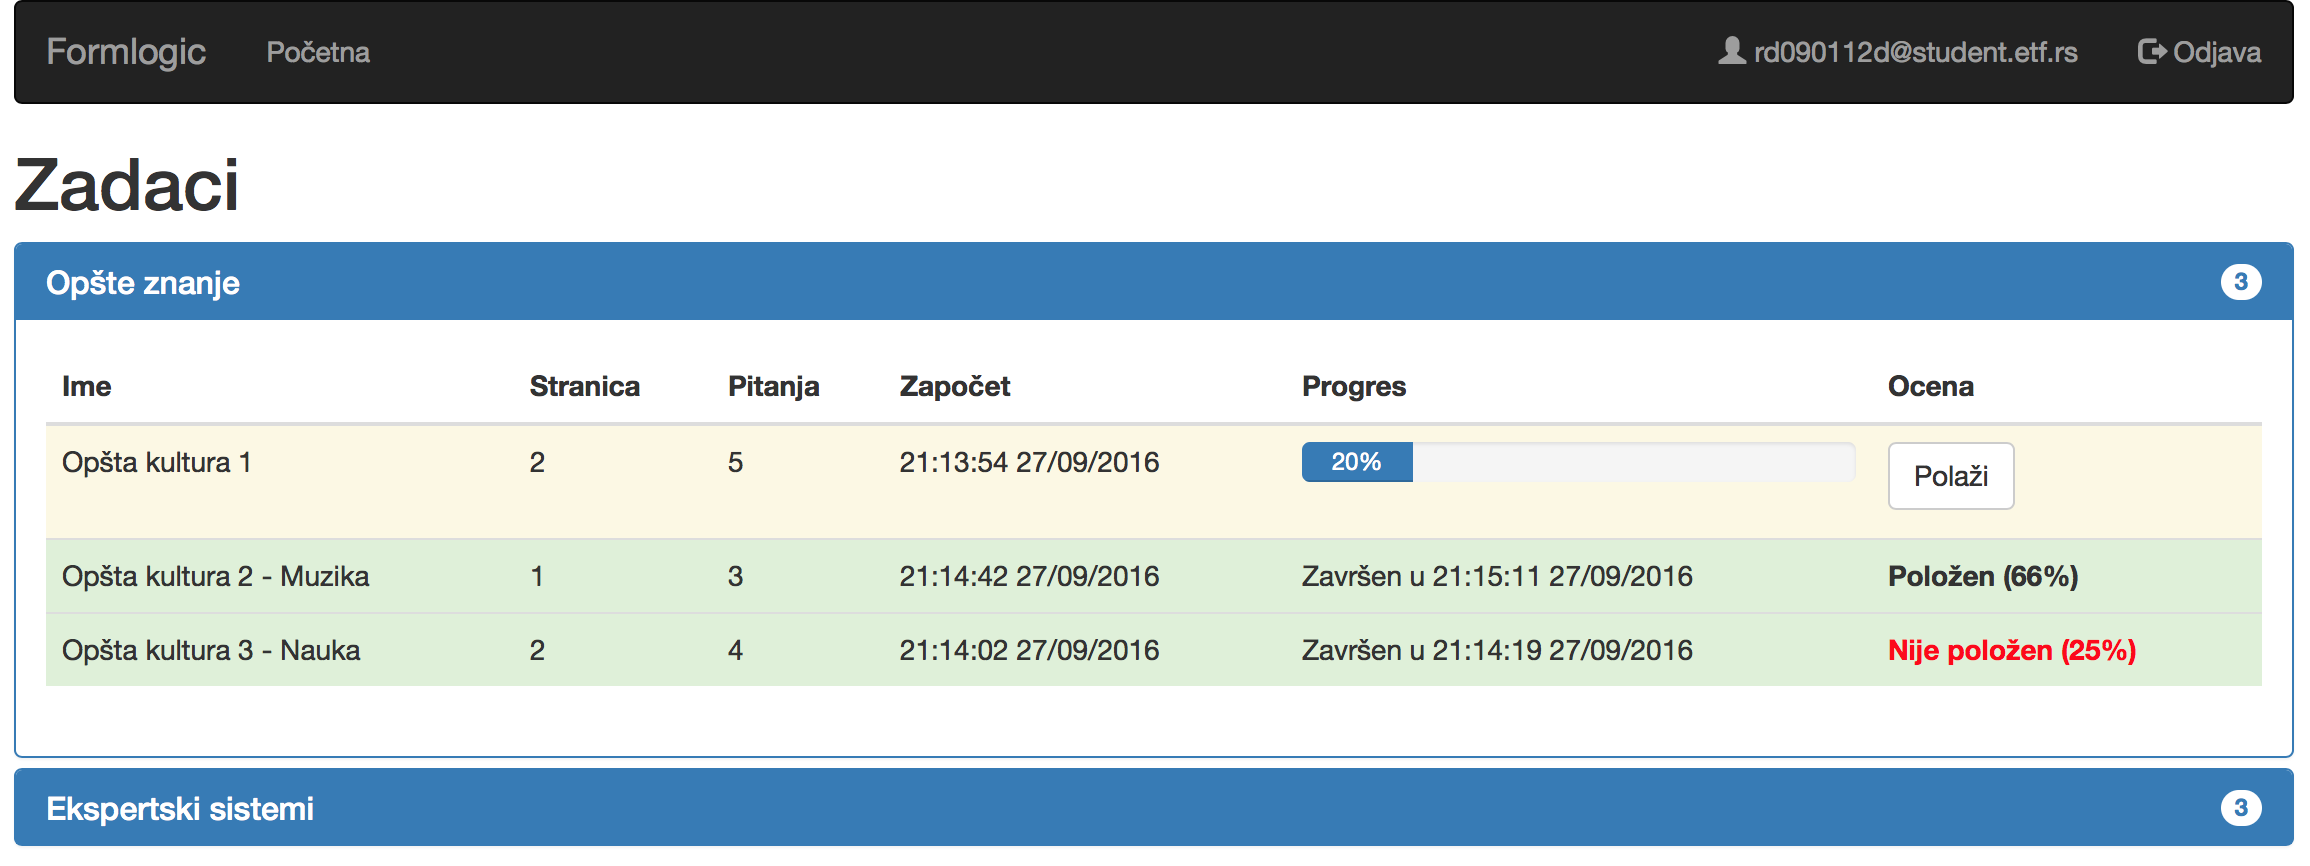
\includegraphics[width=\textwidth]{assignments-collapsed-progress}
\caption{\textit{Gore}: stranica sa zadacima nakon što je sadržaj prve kategorije proširen, za korisnika koji nije polagao nijedan test, \textit{dole}: stranica sa zadacima sa prvim testom u toku, položenim drugim testom i nepoloženim trećim testom}
\label{fig:assignments-collapsed}
\end{figure}

Nakon što korisnik klikne na dugme \textbf{Polaži}, prikazuje mu se prva stranica sa pitanjima odabranog testa. Kada korisnik prvi put otvori stranicu sa pitanjima nekog testa, smatra se da je otpočeo proces izrade tog testa, te će unos u tabeli testova za taj test od tada biti označen žutom pozadinom.

\subsection{Stranica sa pitanjima}
URI stranice sa pitanjima je sledećeg oblika: \path{/user/progress/<assignment-id>/<page-ord>} gde je \texttt{assignment-id} ID zadatka, a \texttt{page-ord} redni broj stranice sa pitanjima tog zadatka. Redni brojevi stranica počinju od broja 1.

Stranica sa pitanjima sastoji se od tri dela (slika \ref{fig:task}). Prvi deo je zaglavlje stranice, na kome se nalazi ime testa, redni broj trenutne stranice sa pitanjima, ukupan broj stranica sa pitanjima u testu i progres popunjavanja testa, u procentima. Progres se računa na osnovu broja popunjenih pitanja, tako da korisnik može da primeti ukoliko je slučajno preskočio neko pitanje sa prethodnih stranica pre nego što preda test.
\begin{figure}[h]
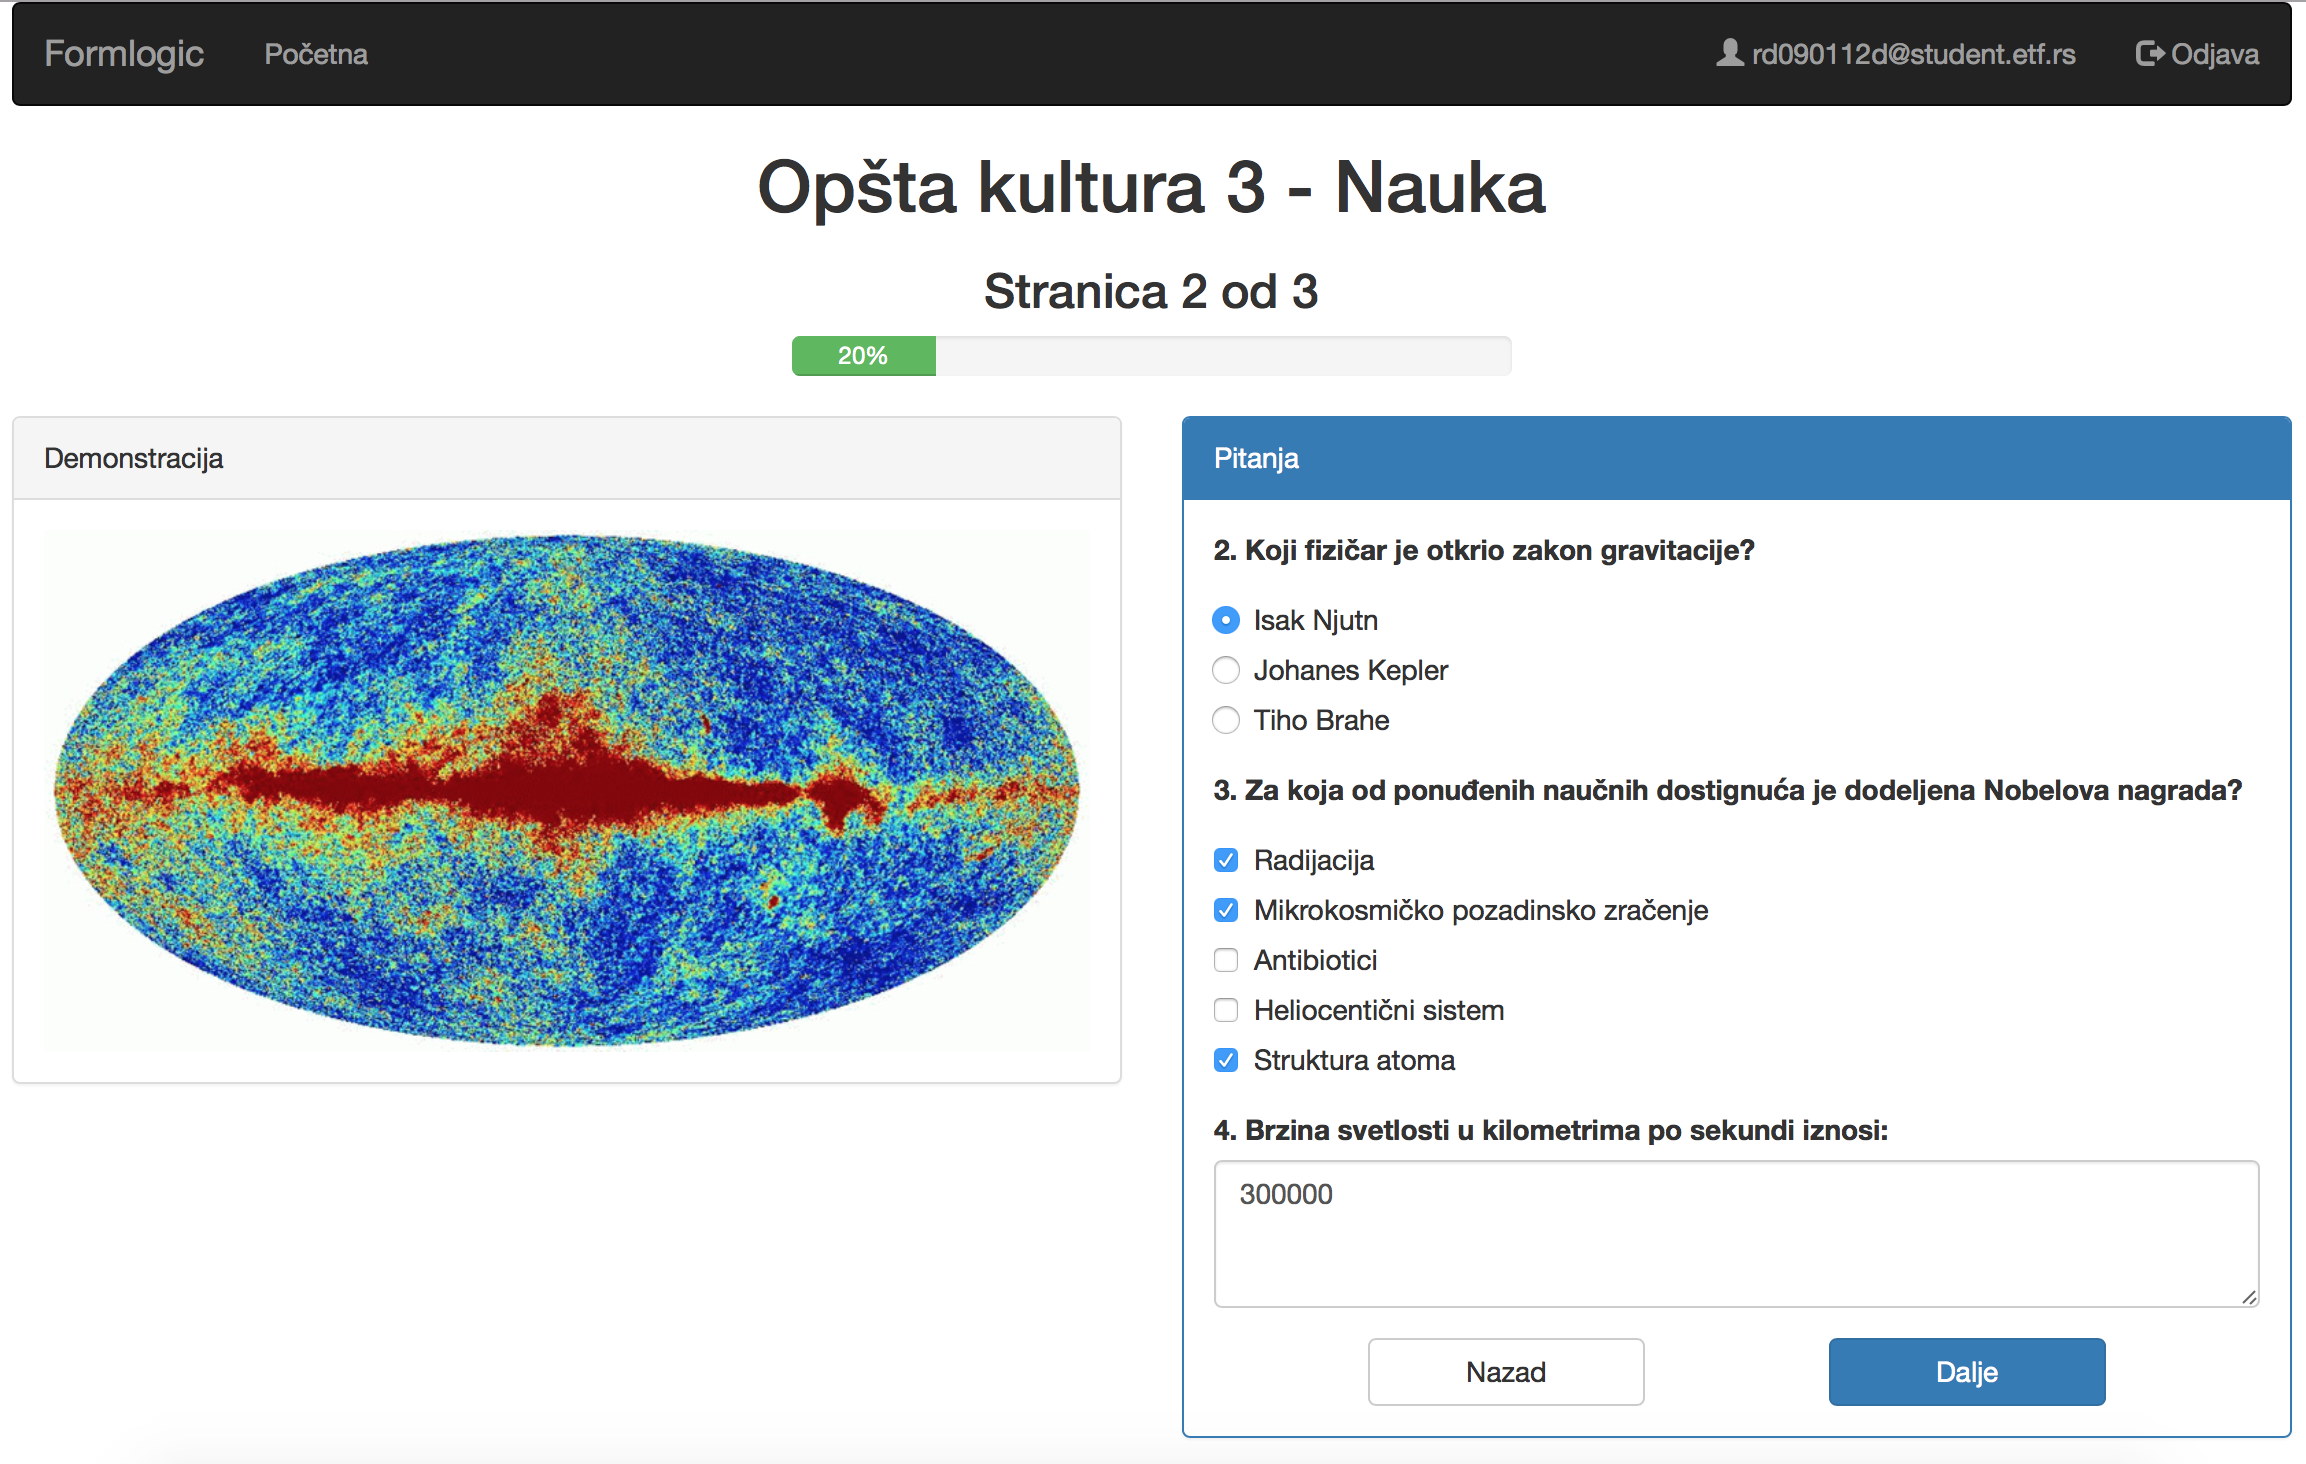
\includegraphics[width=\textwidth]{task}
\caption{Izgled stranice sa pitanjima sa popunjenim odgovorima}
\label{fig:task}
\end{figure}

Drugi deo stranice sa pitanjima je deo sa demonstracijom. Ovaj opcioni deo se nalazi u panelu sa leve strane i sadrži proizvoljan sadržaj. Sadržaj se može specificirati za svaku stranicu sa pitanjima ponaosob, i unosi se direktno u bazu, zajedno sa ostalim informacijama vezanim za konkretni test. Sadržaj se navodi kao deo izvornog koda u Clojure-u, koji se interpretira i renderuje zajedno sa ostatkom HTML stranice, tako da je ovim putem moguće vršiti i složenije operacije nad sadržajem koji treba prikazati.

Treći deo stranice sa pitanjima su sama pitanja. Ona se nalaze u panelu sa desne strane. Na jednoj stranici sa pitanjima moguće je imati proizvoljan broj pitanja. Pitanja su navedena jedna ispod drugog, u rastućem redosledu rednog broja pitanja. Kada se stranica učita, odgovor na svako pitanje je nepopunjen. Kada korisnik jednom odgovori na pitanja sa jednim ili više ponuđenih odgovora, više nije u mogućnosti da poništi svoj odgovor i vrati pitanje u nepopunjeno stanje. Nakon svih pitanja, na dnu panela se nalaze dva dugmeta: \textbf{Nazad} i \textbf{Dalje}. Prvo dugme služi da se korisnik vrati na prethodnu stranicu sa pitanjima, a potonje dugme služi da se ode na sledeću stranicu sa pitanjima. U oba slučaja se čuvaju odgovori koje je korisnik dao na trenutnoj stranici.

Kada se korisnik nađe na poslednjoj stranici sa pitanjima, na dnu stranice pojavljuje se dugme \textbf{Predaj}. Nakon pritiska na ovo dugme korisniku se prikazuje modalni dijalog koji upozorava na to da akcija predavanja testa ne može da se poništi, dajući korisniku još jednu šansu da proveri svoje odgovore (slika \ref{fig:test-submit}. Ukoliko korisnik u pomenutom dijalogu potvrdi akciju predaje, test se smatra završenim, a korisnik se vraća na stranicu sa pregledom testova. Od ovog trenutka korisnik više nije u mogućnosti da menja odgovore na pitanja ovog testa, niti da ga ponovo polaže.

Ukoliko korisnik prekine polaganje u bilo kom trenutku, na primer tako što zatvori prozor pregledača ili ode na neku drugu internet stranicu, može nastaviti sa polaganjem tako što će izabrati test čije je polaganje prekinuo sa stranice sa pregledom testova. Dotadašnji progres, tj. odgovori koje je korisnik dao pre nego što je prekinuo polaganje, će biti restaurirani.
\begin{figure}[h]
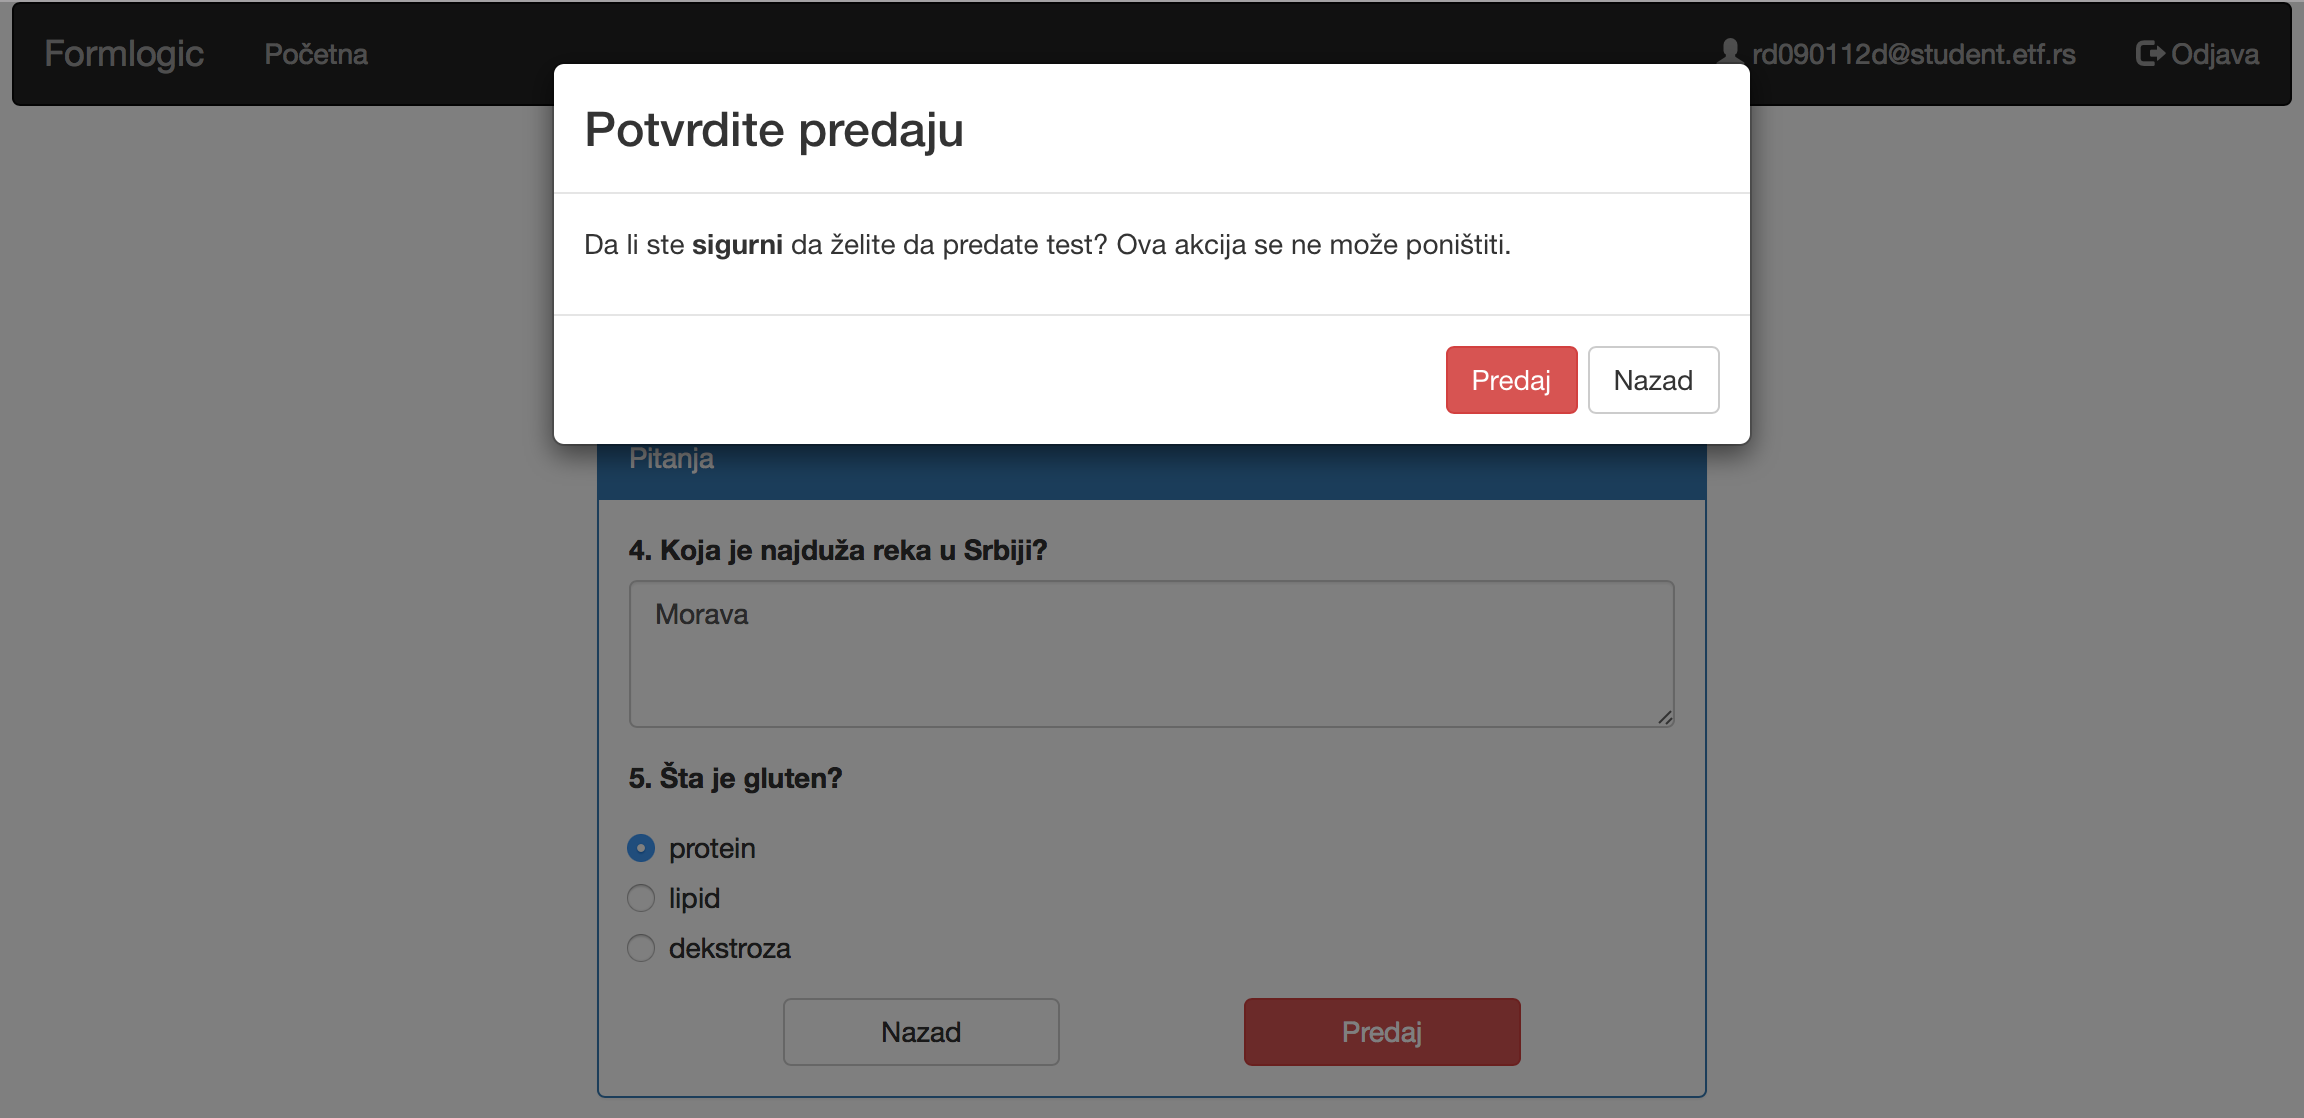
\includegraphics[width=\textwidth]{task-submit}
\caption{Izgled dijaloga za potvrdu predaje testa}
\label{fig:task-submit}
\end{figure}